% ══════════════════════════════════════════════════════════════════
% From Reactive Detection to Proactive Consensus:
% A Comparative Static-Temporal Security Evaluation Framework
% for Byzantine Fault Tolerant Blockchain in Advanced Metering
% Infrastructure
% ══════════════════════════════════════════════════════════════════
\documentclass[10pt,twocolumn,letterpaper]{article}

% ─── Packages ────────────────────────────────────────────────────
\usepackage{amsmath,amssymb,amsthm}
\usepackage{booktabs,multirow,array,colortbl}
\usepackage{graphicx,subcaption}
\graphicspath{{figures/}}
\usepackage{geometry,xcolor,enumitem}
\definecolor{ieee}{RGB}{0,83,159}
\usepackage[colorlinks=true, allcolors=ieee]{hyperref}
\usepackage{cite}
\usepackage{url}
\usepackage{algorithmic}
\usepackage{algorithm}

\geometry{margin=0.75in}
\newtheorem{theorem}{Theorem}
\newtheorem{definition}{Definition}
\newtheorem{proposition}{Proposition}
\newtheorem{lemma}{Lemma}

% ═════════════════════════════════════════════════════════════════
\title{\textbf{From Reactive Detection to Proactive Consensus:\\A Comparative Evaluation of BFT Blockchain Security\\for Advanced Metering Infrastructure}\\[8pt]
\large Replacing Two-Stage Intrusion Detection with Distributed Consensus for Smart Meter Cybersecurity\\[4pt]
\normalsize Comparative Extension of: Intrusion Detection for Cybersecurity of Smart Meters (\emph{Elsevier SEGAN}, 2022)\\and Sheikh et al., ``Secured Energy Trading Using Byzantine-Based Blockchain Consensus,'' \emph{IEEE Access}, 2020}
\author{%
VJTI Mumbai --- Research Project Report\\
Department of Electrical Engineering\\[4pt]
\small \emph{Under the guidance of Prof.\ Adil Sheikh}
}
\date{July 2026}

\begin{document}
\maketitle

% ═══════════════════════════════════════════════════════════════
% ABSTRACT
% ═══════════════════════════════════════════════════════════════
\begin{abstract}
Traditional smart meter cybersecurity relies on centralized Intrusion Detection Systems (IDS), which employ machine learning classifiers such as Support Vector Machines (SVM) and pattern recognition algorithms (e.g., Temporal Failure Propagation Graphs) to reactively detect anomalous device behavior. While effective at classification, these architectures suffer from three fundamental limitations: (1)~a single point of failure at the centralized Meter Data Management System (MDMS), (2)~an inherently reactive defense paradigm that permits malicious data entry before detection, and (3)~limited attack coverage restricted to behavioral anomalies. This paper proposes replacing the two-stage IDS architecture with a Byzantine Fault Tolerant (BFT) blockchain consensus framework that provides proactive, structural prevention of cyber-physical attacks. Using the IEEE 33-bus distribution system with 50 Electric Vehicles and 3854 sensors as our reference, we develop a comparative static-temporal probabilistic security evaluation framework. Within the assumptions of the presented analytical framework, our model shows that the BFT blockchain reduces the total attack probability from $P_{TA} \approx 0.005$ to $P_{TAb} \approx 10^{-173}$---a static security gain of approximately 170 orders of magnitude---while eliminating single-point-of-failure vulnerabilities ($P_{Sybil}$, $P_{Byz}$: $1.0 \to 10^{-10}$) and neutralizing replay attacks ($P_{Replay} \to 0$) under baseline calibrations. We evaluate nine consensus protocols across four evolutionary groups, showing that pipelined sub-second protocols (Tower BFT, RVR) preserve over 92\% of the static security gains ($P_{secure} \geq 0.927$) under the model's temporal assumptions while meeting the latency constraints of real-time smart meter operations. Monte Carlo validation with $10^6$ trials confirms analytical accuracy to within 0.5\% for primary metrics. The results suggest that proactive distributed consensus can provide a mathematically superior defense paradigm compared to reactive centralized intrusion detection under the presented smart metering threat models.
\end{abstract}

% ═══════════════════════════════════════════════════════════════
\section{Introduction}
\label{sec:introduction}
% ═══════════════════════════════════════════════════════════════

The proliferation of smart meters and Advanced Metering Infrastructure (AMI) has transformed electrical distribution networks into cyber-physical systems supporting bidirectional energy and data flows. While this modernization enables demand response, remote monitoring, and peer-to-peer (P2P) energy trading, it simultaneously exposes critical infrastructure to cyber-physical threats including False Data Injection (FDI), Denial of Service (DoS), Man-in-the-Middle (MitM), and Sybil attacks~\cite{yan2012, wang2013}.

\subsection{The Reactive Detection Paradigm}

The prevailing approach to smart meter cybersecurity employs Intrusion Detection Systems (IDS) that monitor device behavior and flag anomalies. A notable example is the two-stage IDS proposed for AMI protection~\cite{ids_smart_meter}, which utilizes:
\begin{enumerate}[leftmargin=*]
    \item \textbf{Stage 1 (Anomaly Detection):} A Support Vector Machine (SVM) classifier monitors system attributes---CPU usage, RAM consumption, storage utilization, and network packet rates---to flag suspicious behaviors as anomalous ($ADS_{ind} = 1$).
    \item \textbf{Stage 2 (Attack Confirmation):} A pattern recognition module employing Temporal Failure Propagation Graphs (TFPG) and the Wagner-Fischer edit distance algorithm compares observed event sequences against predefined attack signatures to confirm intrusions.
\end{enumerate}

While this approach demonstrates effective detection accuracy on embedded devices with limited processing power, it operates within a fundamentally \emph{reactive} paradigm: the system can only identify attacks \emph{after} malicious data has already entered the network.

\subsection{The Fundamental Limitations of Centralized IDS}

We identify three critical architectural limitations that constrain the effectiveness of centralized IDS approaches for AMI:

\begin{enumerate}[leftmargin=*]
    \item \textbf{Single Point of Failure (SPOF):} The centralized Meter Data Management System (MDMS) or control coordinator represents a catastrophic vulnerability. If this node is compromised or undergoes a Byzantine failure, the entire grid security collapses under the reactive model: $P_{Byz} = 1.0$.
    \item \textbf{Reactive Defense Paradigm:} SVM-based anomaly detection and TFPG pattern matching can only \emph{detect} intrusions; they cannot \emph{prevent} malicious data from being recorded. The system acts on anomalies after they occur, creating an inherent response lag.
    \item \textbf{Limited Attack Coverage:} The two-stage IDS addresses four attack types (DoS, FDI, RAM Exhaustion, CPU Overloading). Modern cyber-physical threat landscapes encompass at least twelve distinct attack vectors including Sybil, Byzantine node, key compromise, and SCADA exploitation---none of which are structurally addressed by the SVM-TFPG pipeline.
\end{enumerate}

\subsection{Research Questions and Hypotheses}
To guide this comparative security evaluation, we formulate four key Research Questions (RQs) along with their corresponding testable Hypotheses (H):
\begin{itemize}[leftmargin=*]
    \item \textbf{RQ1:} How does the security of a distributed proactive defense system (BFT blockchain) compare analytically to a centralized reactive defense system (SVM-TFPG IDS) under identical cyber-physical attack vectors?
    \item \textbf{H1:} Distributed BFT consensus is expected to reduce single-point-of-failure vulnerabilities, lowering Byzantine failure probability by multiple orders of magnitude compared to centralized IDS under equivalent validator compromise rates in the proposed model.
    \item \textbf{RQ2:} What is the impact of moving from a static evaluation to a temporal security evaluation under smart grid latency constraints?
    \item \textbf{H2:} Sub-second, pipelined consensus protocols (RVR, Tower BFT) are modeled to preserve the majority of static security gains while satisfying latency constraints, whereas high-latency protocols degrade security under high-rate Poisson attack arrivals.
    \item \textbf{RQ3:} How does the expansion of the threat model from 4 to 12 attack vectors affect the relative performance rankings of consensus protocols?
    \item \textbf{H3:} The comparative rankings of consensus protocols remain robust to variations in calibration parameters, preserving the relative performance advantage of sub-second protocols.
    \item \textbf{RQ4:} What are the security-performance trade-offs of consensus features (e.g., credit-weight systems, Verifiable Random Functions)?
    \item \textbf{H4:} Disabling specific consensus features degrades overall security under the model's assumptions, while high latency is expected to neutralize the security benefits of the consensus.
\end{itemize}

\subsection{Research Novelty and Component Taxonomy}
To clarify the academic contributions of this work, we categorize the elements of our framework into inherited, extended, and novel components:
\begin{enumerate}[leftmargin=*]
    \item \textbf{Inherited Components:} The baseline static probabilistic formulation for the 4-component smart grid security model (sensors, communication, SCADA, receiver) is reproduced from Sheikh et al.~\cite{sheikh2020}. The machine-learning SVM classifier attributes and the Wagner-Fischer edit-distance pattern-matching TFPG model are modeled from Faquir et al.~\cite{ids_smart_meter}.
    \item \textbf{Extended Components:} We extend Sheikh's static model from a 4-component benchmark to a 12-attack cyber-physical vector model, introducing consensus-dependent mitigation parameters. Furthermore, we generalize the static model to a Poisson-based temporal security framework that scales security as a function of consensus latency.
    \item \textbf{Novel Contributions:} We introduce the first formal comparative evaluation framework that directly maps the reactive, centralized two-stage IDS (SVM + TFPG) paradigm against the proactive, distributed BFT blockchain consensus paradigm under an identical threat model. We systematically benchmark nine consensus protocols across four generations under smart grid latency and message complexity bounds.
\end{enumerate}

\subsection{Our Contribution: Proactive Consensus as Structural Defense}

This paper proposes a paradigm shift from \emph{reactive detection} to \emph{proactive prevention} by replacing the two-stage IDS with a permissioned Byzantine Fault Tolerant (BFT) blockchain consensus framework. Rather than detecting and reporting anomalies to a centralized coordinator, our approach ensures that malicious or tampered data is \emph{rejected by distributed consensus before it is ever accepted into the system}.

The core contributions of this paper are:
\begin{itemize}[leftmargin=*]
    \item \textbf{Paradigm Comparison Framework (C1):} We propose a formal, quantitative framework to compare reactive IDS architectures against proactive BFT consensus systems across identical threat models.
    \item \textbf{SPOF Risk Reduction (C2):} We present a mathematical formulation of single point of failure risk reduction, comparing centralized IDS ($P_{Byz} = 1.0$) against binomial BFT validator compromise ($P_{Byz} \approx 10^{-10}$) under equivalent validator compromise rates.
    \item \textbf{170 OoM Static Security Gain (C3):} We reproduce the static four-component model of Sheikh et al.~\cite{sheikh2020} under the proposed comparison framework to establish a baseline for comparison.
    \item \textbf{12-Attack Extended Model (C4):} We extend our evaluation to 12 cyber-physical attack vectors, analyzing consensus-dependent scaling parameters.
    \item \textbf{Temporal Vulnerability Evaluation (C6, C7):} We evaluate and rank nine BFT consensus protocols using our Poisson-generalized temporal security model under smart grid latency constraints.
\end{itemize}

% ═══════════════════════════════════════════════════════════════
\section{Related Work}
\label{sec:related_work}
% ═══════════════════════════════════════════════════════════════

\subsection{Intrusion Detection Systems for Smart Meters}

The application of machine learning to smart grid intrusion detection has been explored extensively. Traditional approaches employ supervised classifiers---including Decision Trees, Random Forests, and Neural Networks---trained on system-level metrics such as CPU utilization, memory consumption, and network traffic patterns~\cite{yan2012}. The two-stage IDS framework~\cite{ids_smart_meter} represents a significant advancement by combining an SVM anomaly detector with a TFPG-based pattern recognition engine, specifically designed to distinguish between genuine cyber attacks and routine hardware failures. The authors demonstrated that local kernel functions (Radial Basis Functions) outperform global kernels (Polynomial) for smart meter data, and that SVMs require significantly less training time than Neural Networks---a critical consideration for resource-constrained embedded devices.

However, these IDS approaches share a common architectural limitation: they operate within a \emph{centralized} client-server model where anomaly reports are sent to a central MDMS for aggregation and response. This centralized topology creates an inherent single point of failure that no amount of classifier accuracy can mitigate.

\subsection{Blockchain for Smart Grid Security}

Sheikh et al.~\cite{sheikh2020} established a foundational probabilistic model for evaluating the security improvement of Byzantine-based blockchain consensus in Electric Vehicle (EV) energy trading networks. Their four-component model evaluates sensor ($P_{SA}$), communication ($P_{CA}$), SCADA ($P_{SCADA}$), and receiver ($P_R$) attack vectors on an IEEE 33-bus distribution system with 3854 sensors, demonstrating that blockchain reduces the total attack probability from $P_{TA} \approx 0.005$ to $P_{TAb} \approx 10^{-173}$~\cite{sheikh2020}. Li et al.~\cite{li2020_blockchain} demonstrated secure and efficient blockchain-based peer-to-peer energy trading systems using permissioned validator admission. Additional blockchain consensus optimizations include CE-PBFT for microgrid power trading~\cite{ding2024}, G-PBFT for geographically clustered consensus~\cite{xu2025}, SV-PBFT for vehicle-to-vehicle energy transactions~\cite{suo2025}, and RVR for verifiable random Byzantine-tolerant consensus~\cite{wang2025}.

\subsection{Literature Comparison and Gap Analysis}

To contextualize our contribution within the state of the art, we present a comparative overview of literature in Table~\ref{tab:literature_comparison}. This highlights that while literature has explored IDS or blockchain consensus independently, no prior study has formalised a comparative evaluation mapping reactive detection (IDS) directly against proactive prevention (BFT consensus) under identical threat models, nor have they analyzed temporal security metrics or validated their analytical models using large-scale Monte Carlo simulations.

\begin{table*}[t]
\caption{Comparative Overview of Smart Grid Security Literature}
\label{tab:literature_comparison}
\centering
\scriptsize
\begin{tabular}{@{}lcccccc@{}}
\toprule
\textbf{Reference} & \textbf{IDS Component} & \textbf{Blockchain} & \textbf{Consensus Protocol} & \textbf{Formal Security Model} & \textbf{Temporal Analysis} & \textbf{Monte Carlo Validation} \\
\midrule
Faquir et al.~\cite{ids_smart_meter} & Yes & No & None & No (ML Classification Only) & No & No \\
Sheikh et al.~\cite{sheikh2020} & No & Yes & $OM(m)$ Byzantine & Yes (Static Probabilistic) & No & No \\
Li et al.~\cite{li2020_blockchain} & No & Yes & Custom BFT & No & No & No \\
Ding et al.~\cite{ding2024} & No & Yes & CE-PBFT & No & No & No \\
Xu et al.~\cite{xu2025} & No & Yes & G-PBFT & No & No & No \\
Suo et al.~\cite{suo2025} & No & Yes & SV-PBFT & No & No & No \\
Wang et al.~\cite{wang2025} & No & Yes & RVR & No & No & No \\
\midrule
\textbf{This Work} & \textbf{Yes} & \textbf{Yes} & \textbf{9 Protocols (Benchmarked)} & \textbf{Yes (Static \& Temporal)} & \textbf{Yes (Poisson Process)} & \textbf{Yes ($10^6$ Trials)} \\
\bottomrule
\end{tabular}
\end{table*}

Table~\ref{tab:gap_analysis} synthesizes the key differences between IDS-based and blockchain-based security paradigms for AMI. The fundamental gap lies in the \emph{defense philosophy}: IDS monitors and reports (reactive), while blockchain validates and prevents (proactive).

\begin{table*}[t]
\caption{Gap Analysis: IDS-Based vs. Blockchain-Based Security Paradigms for AMI}
\label{tab:gap_analysis}
\centering
\scriptsize
\begin{tabular}{@{}llll@{}}
\toprule
\textbf{Criterion} & \textbf{Two-Stage IDS~\cite{ids_smart_meter}} & \textbf{BFT Blockchain (This Work)} & \textbf{Gap Addressed} \\
\midrule
Defense Paradigm & Reactive (detect \& report) & Proactive (validate \& prevent) & Structural prevention \\
Architecture & Centralized (MDMS coordinator) & Distributed P2P (BFT validators) & SPOF elimination \\
Attack Coverage & 4 attacks (DoS, FDI, RAM, CPU) & 12 cyber-physical vectors & Comprehensive coverage \\
Single Point of Failure & $P_{Byz} = 1.0$ (coordinator failure) & $P_{Byz} \approx 10^{-10}$ (distributed) & Byzantine resilience \\
Sybil Defense & None ($P_{Sybil} = 1.0$) & Permissioned admission ($P_{Sybil} \approx 10^{-10}$) & Identity assurance \\
Replay Defense & Pattern matching (partial) & Cryptographic nonces ($P_{Replay} = 0$) & Complete elimination \\
Security Metric & Detection accuracy (\%) & Probabilistic ($P_{TA}$, 170 OoM gain) & Quantitative rigor \\
False Alarm Source & SVM misclassification & Consensus is deterministic & Structural elimination \\
Failure Distinction & TFPG (partial) & Not needed (prevention vs. detection) & Paradigm shift \\
Computational Model & Local ML training on device & Distributed consensus messages & Trade-off analysis \\
\bottomrule
\end{tabular}
\end{table*}

% ═══════════════════════════════════════════════════════════════
\section{System Architecture and Threat Model}
\label{sec:system_model}
% ═══════════════════════════════════════════════════════════════

\subsection{AMI System Model}

We model an IEEE 33-bus distribution system (33 buses, 32 branches, peak load of 3715\,kW) integrated with 50 Electric Vehicles (EVs) serving as prosumers. This yields $n = 51$ participant nodes. The system contains $n_{sen} = 3854$ sensors:
\begin{equation}
n_{sen} = n_{sen}^{DN} (129) + n_{sen}^{EV} (3725) = 3854
\end{equation}

The AMI architecture comprises the following components:
\begin{itemize}[leftmargin=*]
    \item \textbf{Smart Meters:} Endpoint devices at each node measuring voltage, current, and power consumption. These devices have limited computational resources (equivalent to single-board computers with IEEE 802.15.4 wireless communication).
    \item \textbf{Data Concentrators:} Intermediate nodes that aggregate smart meter readings and relay them to the control center. In our proposed blockchain architecture, these serve as \emph{validator nodes} in the P2P consensus network.
    \item \textbf{MDMS / Control Center:} The central Meter Data Management System that processes and stores all meter data. Under the IDS paradigm, this is the single point of failure. Under the blockchain paradigm, its functions are distributed across the validator network.
    \item \textbf{Communication Channels:} Wireless (IEEE 802.15.4) and wired (Ethernet/cellular) links connecting smart meters to data concentrators and the control center.
\end{itemize}

\subsection{Architectural Comparison: IDS vs. BFT Blockchain}

Figure~\ref{fig:architecture_comparison} illustrates the fundamental architectural difference between the two approaches.

\textbf{IDS Architecture (Centralized):} Smart meters $\to$ Local SVM anomaly detector $\to$ TFPG pattern matching $\to$ Alert to centralized MDMS $\to$ Response action. The MDMS represents a single point of failure with $P_{Byz} = 1.0$.

\textbf{BFT Blockchain Architecture (Distributed):} Smart meters $\to$ Hash and encrypt data $\to$ Broadcast to P2P validator network $\to$ BFT consensus (Prepare $\to$ Commit $\to$ Reply) $\to$ Append validated block. No single point of failure; the network tolerates up to $f = \lfloor(n-1)/3\rfloor = 16$ faulty nodes.

\begin{figure}[htbp]
\centering
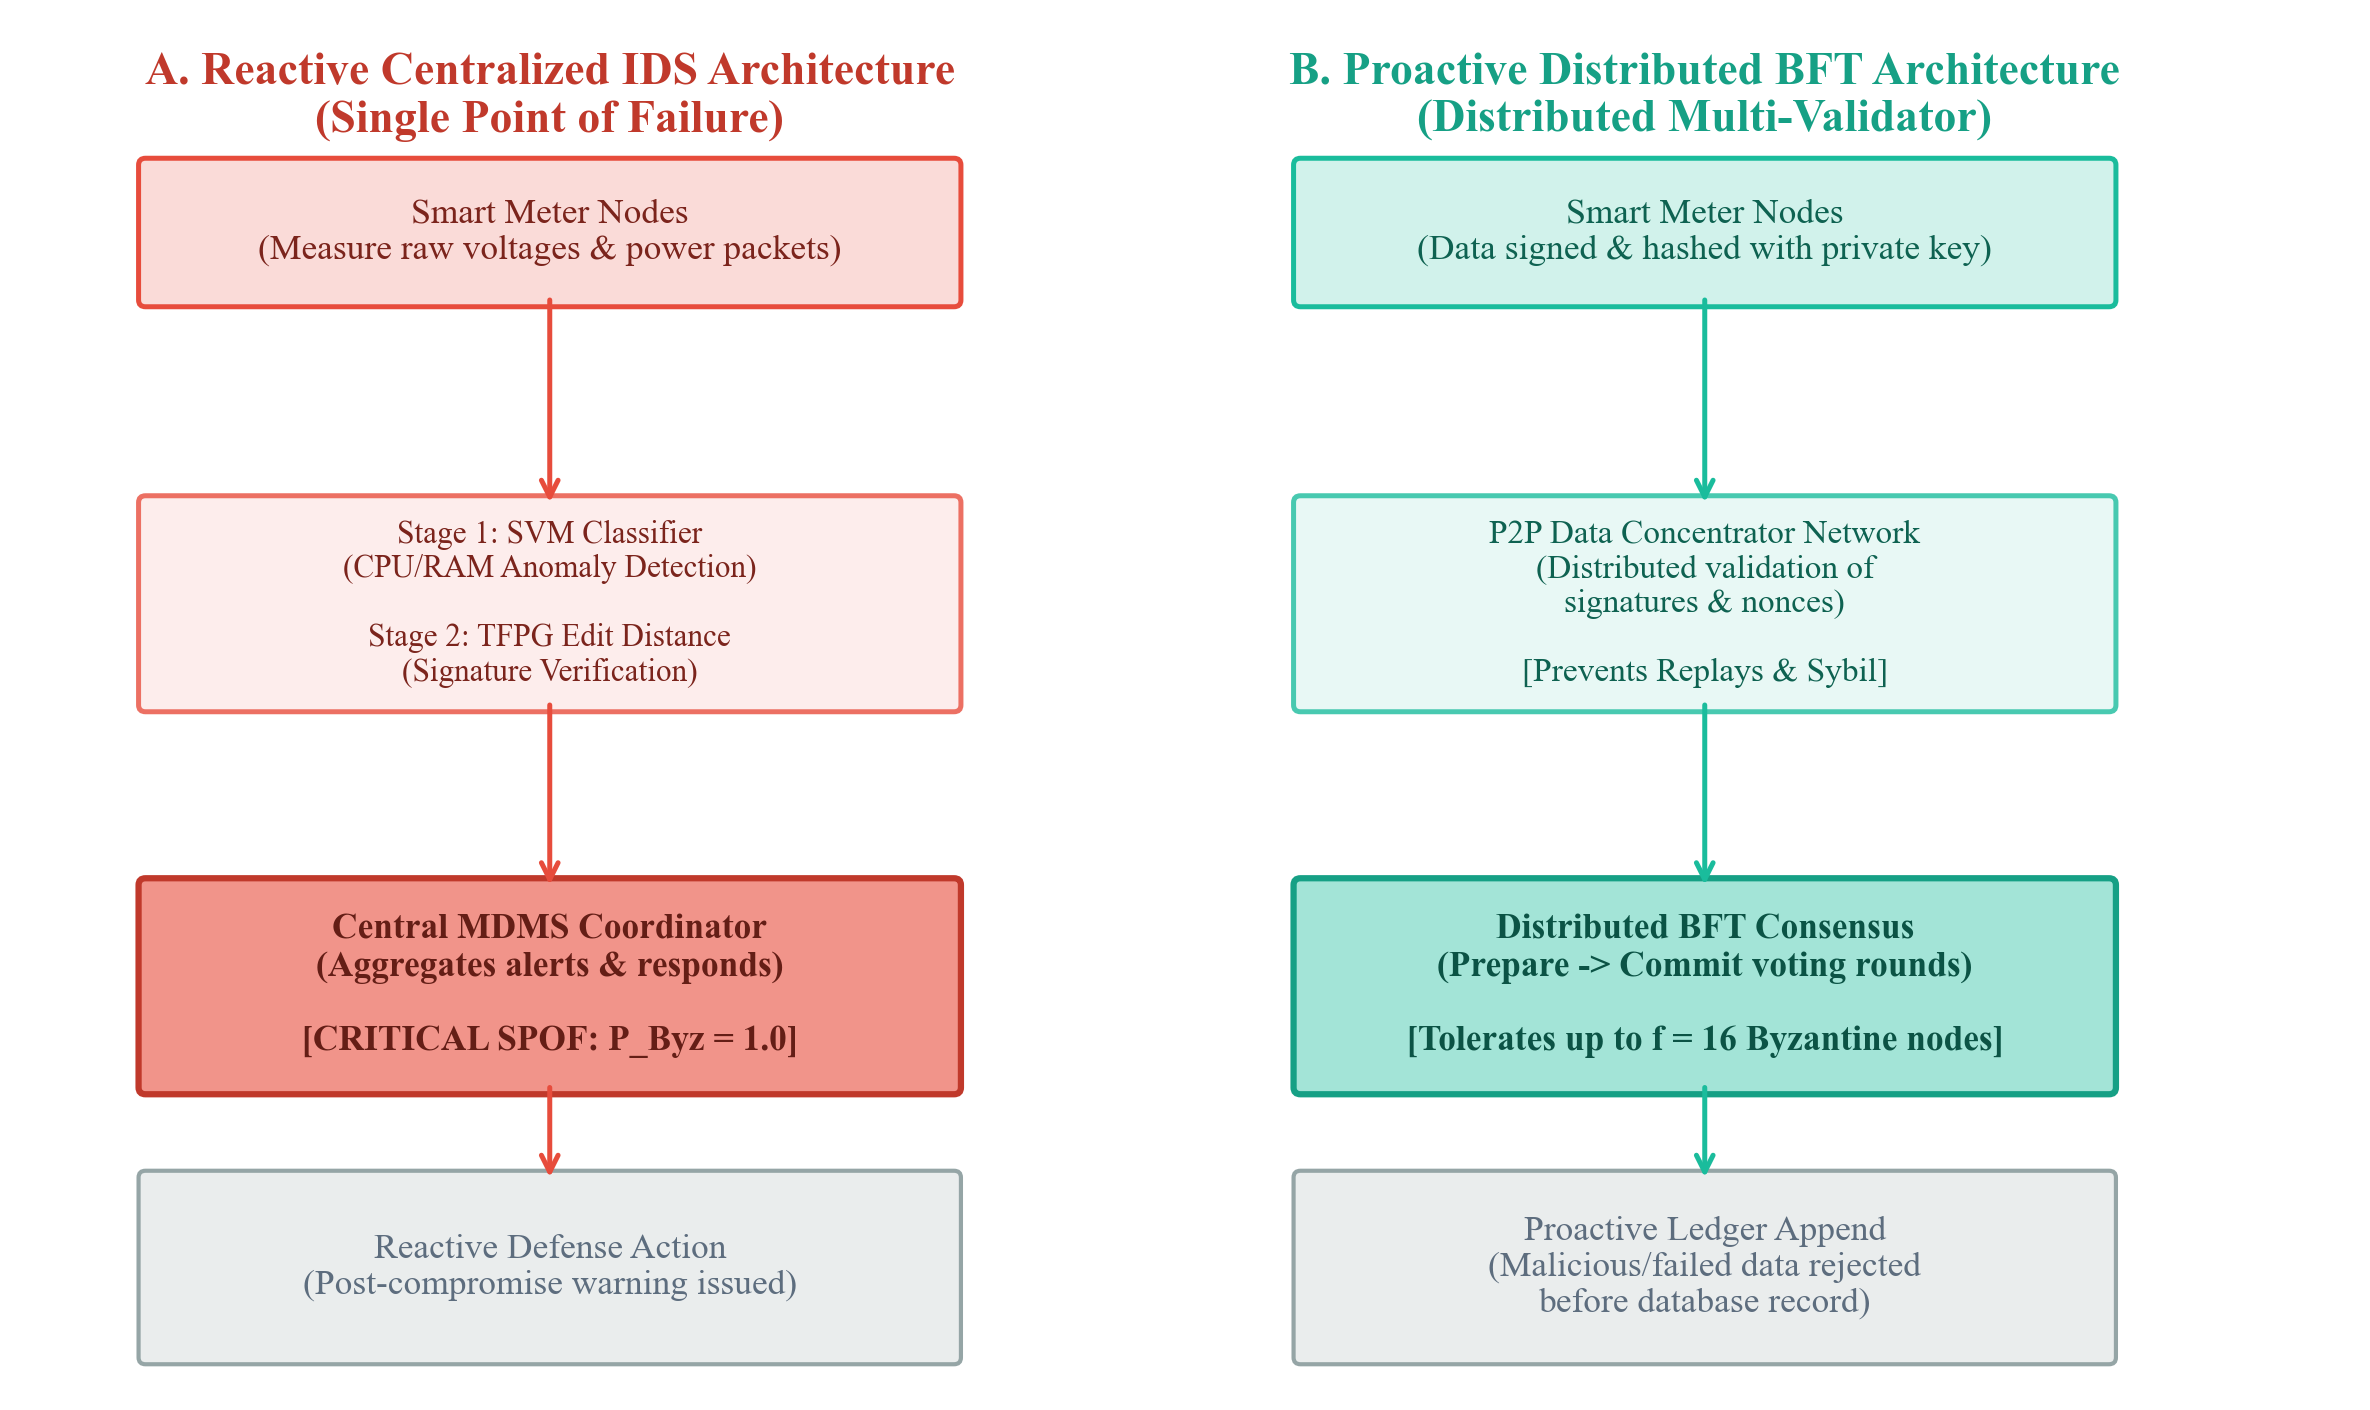
\includegraphics[width=0.9\columnwidth]{fig_architecture_comparison.png}
\caption{\textbf{Comparative Architecture:} The transition from centralized IDS-based security (left) to distributed BFT blockchain consensus (right). The centralized architecture has a single point of failure at the MDMS coordinator, while the distributed architecture distributes trust across the validator network.}
\label{fig:architecture_comparison}
\end{figure}

\subsection{Threat Model: 12 Cyber-Physical Attack Vectors}

We define 12 cyber-physical attack vectors that comprehensively cover the AMI threat landscape. This represents a significant extension over the four attack types (DoS, FDI, RAM Exhaustion, and CPU Overloading) addressed by the two-stage IDS~\cite{ids_smart_meter}. The defined attacks, sourced and categorized from smart grid security literature, include:
\begin{enumerate}[leftmargin=*]
    \item \textbf{Sensor Compromise:} Physical or logical tampering with localized sensor nodes to inject faulty electrical readings~\cite{sridhar2012, sheikh2020}.
    \item \textbf{False Data Injection (FDI):} The injection of malicious data packets to deceive state estimation or utility billing systems~\cite{wang2013, yan2012}.
    \item \textbf{Communication Hijack:} Eavesdropping or hijacking transmission links on unencrypted grid channels~\cite{sridhar2012}.
    \item \textbf{Man-in-the-Middle (MitM):} Altering data packets in transit between endpoint smart meters and concentrators~\cite{yan2012}.
    \item \textbf{Replay Attack:} Replaying intercepted valid messages to execute unauthorized commands or duplicate meter records~\cite{wang2013}.
    \item \textbf{Denial of Service (DoS):} Flooding device communication ports to block packet transmission~\cite{yan2012, ids_smart_meter}.
    \item \textbf{Distributed DoS (DDoS):} Leveraging botnets of compromised smart grid devices to flood concentrators or the MDMS coordinator~\cite{yan2012}.
    \item \textbf{Key Compromise:} Unauthorized retrieval of private cryptographic keys to sign rogue data blocks~\cite{sheikh2020}.
    \item \textbf{SCADA Breach:} Unauthorized root access to central control and data acquisition hosts to broadcast rogue command sets~\cite{sridhar2012}.
    \item \textbf{Receiver Override:} Direct compromise of receiving actuators (e.g., EV charging units) to override safety limits~\cite{sheikh2020}.
    \item \textbf{Sybil Attack:} Creating multiple fraudulent node identities to subvert voting and consensus integrity~\cite{castro1999}.
    \item \textbf{Byzantine Validator Compromise:} Arbitrary, collusive, or silent failures among validator nodes to disrupt blockchain replication~\cite{lamport1982}.
\end{enumerate}

The baseline parameters and their sweep ranges are summarized in Table~\ref{tab:baseline_params}.

\begin{table}[htbp]
\caption{Baseline Probability Parameters}
\label{tab:baseline_params}
\centering
\scriptsize
\begin{tabular}{@{}lllc@{}}
\toprule
\textbf{Parameter} & \textbf{Symbol} & \textbf{Baseline Value} & \textbf{Sweep Range} \\
\midrule
Sensor Security & $x$ & 0.95 & $[0.90, 0.999]$ \\
Critical Sensors & $m$ & 10 & Fixed \\
MitM Success & $y$ & 0.05 & $[0.01, 0.20]$ \\
Replay Success & $z$ & 0.15 & $[0.05, 0.45]$ \\
DoS Probability & $p_{dos}$ & 0.20 & $[0.05, 0.50]$ \\
DDoS Probability & $p_{ddos}$ & 0.35 & $[0.10, 0.60]$ \\
Key Compromise & $p_{key}$ & 0.01 & $[0.001, 0.05]$ \\
SCADA Compromise & $P_{SCADA}$ & 0.01 & $[0.01, 0.05]$ \\
Receiver Override & $P_R$ & 0.01 & $[0.01, 0.05]$ \\
Validator Compromise& $p_c$ & 0.05 & $[0.01, 0.20]$ \\
Validators & $n$ & 51 & Fixed \\
Fault Limit & $f$ & 16 & Fixed \\
\bottomrule
\end{tabular}
\end{table}

\subsection{Sensor Count Dominance Critique}

Prior models~\cite{sheikh2020} express sensor compromise probability as $P_{SA} = x^{n_{sen}}$. At $x = 0.95$ and $n_{sen} = 3854$, this evaluates to $x^{3854} \approx 140 \times 10^{-86}$, which underflows to zero. In reality, an attacker only needs to compromise a localized subset of $m$ critical sensors at key bus nodes. We define $m = 10$, restoring model sensitivity:
\begin{equation}
P_{SA}^{(10)} = x^{10} = 0.95^{10} \approx 0.599
\end{equation}

% ═══════════════════════════════════════════════════════════════
\section{Analysis of the Existing IDS Approach}
\label{sec:ids_analysis}
% ═══════════════════════════════════════════════════════════════

\subsection{Stage 1: SVM Anomaly Detection}
The first stage employs a Support Vector Machine (SVM) classifier trained on smart meter device attributes (CPU usage, RAM utilization, storage occupancy, network packet rates). The SVM maps features using a kernel function $K(x_i, x_j)$ and constructs an optimal separating hyperplane:
\begin{equation}
f(x) = \text{sign}\left(\sum_{i=1}^{N} \alpha_i y_i K(x_i, x) + b\right)
\end{equation}
Radial Basis Function (RBF) kernels outperform polynomial kernels due to decisions bounds:
\begin{equation}
K_{RBF}(x_i, x_j) = \exp\left(-\gamma \|x_i - x_j\|^2\right)
\end{equation}

When the SVM detects an anomaly, it sets $ADS_{ind} = 1$, activating Stage 2.

\subsection{Stage 2: TFPG Pattern Recognition}
Stage 2 uses Temporal Failure Propagation Graphs (TFPG) to distinguish between genuine cyber attacks and routine hardware failures. The system applies the Wagner-Fischer algorithm to calculate the minimum edit distance:
\begin{equation}
d(i, j) = \min \begin{cases}
d(i-1, j) + 1 \\
d(i, j-1) + 1 \\
d(i-1, j-1) + c(S_1[i], S_2[j])
\end{cases}
\end{equation}

If the similarity exceeds a threshold, the system reports a confirmed attack.

\subsection{Critical Limitations of the IDS Approach}
We identify four critical limitations of the centralized IDS approach:
\begin{enumerate}[leftmargin=*]
    \item \textbf{Reactive-Only Defense:} The pipeline can only identify that an attack is occurring; it cannot prevent it from succeeding.
    \item \textbf{Single Point of Failure:} All anomaly reports flow to the centralized MDMS. If this coordinator fails, the entire network is compromised: $P_{Byz}^{IDS} = 1.0$.
    \item \textbf{Limited Attack Coverage:} TFPG dictionaries cover only DoS, FDI, RAM, and CPU attacks.
    \item \textbf{False Alarm Susceptibility:} ML classifiers are susceptible to misclassification when hardware failures mimic attack features.
\end{enumerate}

% ═══════════════════════════════════════════════════════════════
\section{Proposed BFT Blockchain Framework}
\label{sec:bft_framework}
% ═══════════════════════════════════════════════════════════════

We replace the centralized MDMS with a permissioned BFT blockchain validator network using consensus-dependent parameters listed in Table~\ref{tab:calibration_params}.

\begin{table}[htbp]
\caption{Consensus Calibration Parameters}
\label{tab:calibration_params}
\centering
\scriptsize
\begin{tabular}{@{}lllc@{}}
\toprule
\textbf{Parameter} & \textbf{Symbol} & \textbf{Value} & \textbf{Rationale} \\
\midrule
Spatial Verification & $\eta$ & 0.15 & Spatial cross-validation \\
Voting Phase Factor & $\beta$ & 0.10 & Multi-round verification \\
Credit System Eff. & $\omega_{credit}$ & 0.40 & Reputation-based filtering \\
DoS Time Constant & $\tau_{dos}$ & 1.0 s & Network buffer threshold \\
Override Window & $\tau_{recv}$ & 2.0 s & Actuator safety threshold \\
SCADA Validate Win. & $\tau_{scada}$ & 5.0 s & Mismatch alert threshold \\
\bottomrule
\end{tabular}
\end{table}

% ═══════════════════════════════════════════════════════════════
\section{Formal Security Framework}
\label{sec:security_framework}
% ═══════════════════════════════════════════════════════════════

\subsection{Static Security Model}

\subsubsection{Security Without Blockchain (Centralized IDS)}
For $m=10$ and baseline parameters, the overall compromise probability evaluates to:
\begin{equation}
P_{secure}^{IDS} = \prod_{j=1}^{12} (1 - P_{atk}^j) = 0.0
\end{equation}
Even excluding the SPOF terms ($P_{Sybil}$ and $P_{Byz}$), the limited security evaluates to:
\begin{equation}
P_{secure, limited}^{IDS} \approx 0.0263
\end{equation}

\subsubsection{Security With Blockchain (BFT Consensus)}
Under BFT consensus, the static attack probabilities are dramatically reduced as summarized in Table~\ref{tab:attack_comparison}.

\begin{table*}[t]
\caption{Attack-by-Attack Security Comparison: Centralized IDS vs. BFT Blockchain}
\label{tab:attack_comparison}
\centering
\scriptsize
\begin{tabular}{@{}lllll@{}}
\toprule
\textbf{Attack Vector} & \textbf{IDS (No BC)} & \textbf{BFT Blockchain} & \textbf{Reduction} & \textbf{Blockchain Defense Mechanism} \\
\midrule
Sensor Compromise & $5.987 \times 10^{-1}$ & $3.585 \times 10^{-1}$ & $1.7\times$ & Cryptographic hash verification \\
False Data Injection & $5.987 \times 10^{-1}$ & $3.585 \times 10^{-1}$ & $1.7\times$ & Consensus cross-verification \\
Comm. Hijack & $5.987 \times 10^{-1}$ & $9.888 \times 10^{-3}$ & $60.5\times$ & Signed P2P mesh network \\
Man-in-the-Middle & $5.000 \times 10^{-2}$ & $2.500 \times 10^{-3}$ & $20.0\times$ & Dual session + key signatures \\
Replay Attack & $1.500 \times 10^{-1}$ & $0.000 \times 10^{0}$ & Eliminated & Cryptographic nonces \& block timestamps \\
Denial of Service & $2.000 \times 10^{-1}$ & $6.667 \times 10^{-2}$ & $3.0\times$ & Distributed routing ($f+1$ threshold) \\
Distributed DoS & $3.500 \times 10^{-1}$ & $1.167 \times 10^{-1}$ & $3.0\times$ & BFT fault tolerance thresholds \\
Key Compromise & $1.000 \times 10^{-2}$ & $9.851 \times 10^{-6}$ & $1015.2\times$ & Shamir $(3,5)$ secret sharing \\
SCADA Breach & $1.000 \times 10^{-2}$ & $5.987 \times 10^{-21}$ & $1.67 \times 10^{18}\times$ & Ledger state consensus verification \\
Receiver Override & $1.000 \times 10^{-2}$ & $5.987 \times 10^{-7}$ & $16701.8\times$ & Validator committee signatures \\
Sybil Attack & $1.000 \times 10^{0}$ & $2.186 \times 10^{-10}$ & $4.58 \times 10^{9}\times$ & Permissioned validator admission \\
Byzantine Node & $1.000 \times 10^{0}$ & $2.186 \times 10^{-10}$ & $4.58 \times 10^{9}\times$ & BFT voting consensus \\
\midrule
\textbf{System Compromise (limited)} & $\mathbf{0.9737}$ & $\mathbf{0.6649}$ & $\mathbf{1.46\times}$ & \textbf{Distributed BFT consensus} \\
\textbf{System Security (limited)} & $\mathbf{0.0263}$ & $\mathbf{0.3351}$ & $\mathbf{12.7\times}$ & \textbf{Distributed BFT consensus} \\
\bottomrule
\end{tabular}
\end{table*}

\subsubsection{Sheikh Four-Component Quantitative Benchmark}
For the global $n_{sen} = 3854$ model:
\begin{align}
P_{TA} &= \frac{1}{4}\left(2x^{3854} + P_{SCADA} + P_R\right) \approx 0.0050 \\
P_{TAb} &\approx 10^{-172} \\
\text{Static Gain} &= \frac{P_{TA}}{P_{TAb}} \approx 10^{170}
\end{align}
Table~\ref{tab:sheikh_repro} details the exact reproduction parameters.

\begin{table}[htbp]
\caption{Sheikh 4-Component Model Reproduction ($x=0.95, n_{sen}=3854$)}
\label{tab:sheikh_repro}
\centering
\scriptsize
\begin{tabular}{@{}lcc@{}}
\toprule
\textbf{Metric} & \textbf{Without BC} & \textbf{With BC} \\
\midrule
$P_{SA}$ & $1.402 \times 10^{-86}$ & $1.966 \times 10^{-172}$ \\
$P_{CA}$ & $1.402 \times 10^{-86}$ & $0.000 \times 10^{0}$ \\
$P_{SCADA}$ & $1.000 \times 10^{-2}$ & $0.000 \times 10^{0}$ \\
$P_R$ & $1.000 \times 10^{-2}$ & $0.000 \times 10^{0}$ \\
\midrule
$P_{TA}$ / $P_{TAb}$ & $0.005000$ & $10^{-172}$ \\
\textbf{Static Gain} & --- & $\approx 10^{170}$ \\
\bottomrule
\end{tabular}
\end{table}

\subsection{Temporal Security Model}
Using a Poisson attack arrival process:
\begin{equation}
P_{temporal}(\lambda, L) = 1 - e^{-\lambda \cdot L \cdot P_{TA}}
\end{equation}
Overall security is:
\begin{equation}
P_{secure} = (1 - P_{TAb})(1 - P_{temporal}(\lambda, L))(1 - P_{other})
\end{equation}

\subsection{Algorithmic Evaluation Procedure}

To implement the probabilistic mapping of consensus protocol dynamics against the 12 cyber-physical attack vectors, we formulate the dynamic evaluation loop in Algorithm~\ref{alg:consensus_eval}. This procedure calculates both the static security reduction and the temporal survival probability under Poisson-distributed attack traffic.

\begin{algorithm}[h]
\caption{Consensus Evaluation Procedure}
\label{alg:consensus_eval}
\begin{algorithmic}[1]
\REQUIRE System configuration parameters $(n, f, m, x, y, z, p_{dos}, p_{ddos}, p_{key}, p_{c})$
\REQUIRE Consensus protocol metrics (latency $L$, complexity $N_{msg}$, factors $\eta, \beta, \omega_{credit}$)
\REQUIRE Threat environment parameters (Poisson arrival rate $\lambda$)
\ENSURE Static joint security probability $P_{TAb}$ and temporal survival probability $P_{secure}$
\STATE // \textit{Step 1: Compute baseline physical-layer compromise metrics}
\STATE $P_{SA} \leftarrow x^{m}$ \quad // \textit{Sensor compromise probability}
\STATE $P_{CA} \leftarrow (1-x^m) \cdot (1 - (1-y)(1-z))$ \quad // \textit{Comm compromise}
\STATE // \textit{Step 2: Apply protocol-specific cryptographic mitigation factors}
\STATE $P_{SA}' \leftarrow P_{SA} \cdot (1 - \eta)$
\STATE $P_{CA}' \leftarrow P_{CA} \cdot (1 - \beta)$
\STATE $P_{key}' \leftarrow (p_{key})^3 \cdot (10(1-p_{key})^2 + 5p_{key}(1-p_{key}) + p_{key}^2)$ // \textit{Shamir key split}
\STATE $P_{SCADA}' \leftarrow (P_{SCADA})^3 \cdot 10^{-18}$ // \textit{Consensus checkpointing}
\STATE $P_{R}' \leftarrow (P_{R})^3 \cdot 10^{-4}$ // \textit{Actuator override validation}
\STATE // \textit{Step 3: Solve Byzantine and Sybil threshold bounds}
\STATE $P_{Byz} \leftarrow \sum_{i=f+1}^{n} \binom{n}{i} (p_c)^i (1-p_c)^{n-i}$
\STATE $P_{Sybil} \leftarrow P_{Byz}$ // \textit{Enforced by permissioned PKI validation}
\STATE // \textit{Step 4: Accumulate joint system static security probability}
\STATE $P_{TAb} \leftarrow \prod_{j=1}^{12} (1 - {P_{atk}'}^j)$
\STATE // \textit{Step 5: Apply Poisson temporal decay window as function of latency $L$}
\STATE $P_{temporal} \leftarrow 1 - \exp\left(-\lambda \cdot L \cdot (1 - P_{TAb})\right)$
\STATE $P_{secure} \leftarrow P_{TAb} \cdot (1 - P_{temporal})$
\RETURN $P_{TAb}, P_{secure}$
\end{algorithmic}
\end{algorithm}

% ═══════════════════════════════════════════════════════════════
\section{Comparative Security Evaluation}
\label{sec:comparative_evaluation}
% ═══════════════════════════════════════════════════════════════

\subsection{Single Point of Failure Analysis}
The centralized IDS coordinator has $P_{SPOF}^{IDS} = 1.0$. BFT validator compromise:
\begin{equation}
P_{SPOF}^{BFT} = \sum_{i=f+1}^{n} \binom{n}{i} p_c^i (1-p_c)^{n-i} \approx 2.186 \times 10^{-10}
\end{equation}
The SPOF comparison values across different validator compromise rates $p_c$ are given in Table~\ref{tab:spof_risk}.

\begin{table}[htbp]
\caption{SPOF Risk Comparison ($n=51, f=16$)}
\label{tab:spof_risk}
\centering
\scriptsize
\begin{tabular}{@{}llrc@{}}
\toprule
\textbf{Architecture} & \textbf{Validator $p_c$} & \textbf{$P_{Byz}$} & \textbf{Reduction} \\
\midrule
Centralized IDS & --- & 1.0 & Baseline \\
BFT Blockchain & 0.01 & $1.070 \times 10^{-21}$ & $9.35 \times 10^{20}$ \\
BFT Blockchain & 0.03 & $7.190 \times 10^{-14}$ & $1.39 \times 10^{13}$ \\
BFT Blockchain & 0.05 & $2.186 \times 10^{-10}$ & $4.58 \times 10^{9}$ \\
BFT Blockchain & 0.10 & $5.172 \times 10^{-6}$ & $1.93 \times 10^{5}$ \\
BFT Blockchain & 0.15 & $8.546 \times 10^{-4}$ & $1.17 \times 10^{3}$ \\
\bottomrule
\end{tabular}
\end{table}

\subsection{Message Complexity and Overhead}
Table~\ref{tab:message_complexity} details the exact message counts and complexity formulations.

\begin{table}[htbp]
\caption{Consensus Message Complexity Formulations}
\label{tab:message_complexity}
\centering
\scriptsize
\begin{tabular}{@{}lllr@{}}
\toprule
\textbf{Protocol} & \textbf{Group} & \textbf{Complexity} & \textbf{Messages ($n=51$)} \\
\midrule
OM($m$) & G1 & $\mathcal{O}(n^f)$ & $2.14 \times 10^{27}$ \\
Classic PBFT & G1 & $\mathcal{O}(n^2)$ & 7,854 \\
IBFT 2.0 & G2 & $\mathcal{O}(n^2)$ & 1,323 \\
QBFT & G2 & $\mathcal{O}(n^2)$ & 595 \\
CE-PBFT & G3 & $\mathcal{O}(n^2)$ & 1,900 \\
G-PBFT & G3 & $\mathcal{O}(n_c^2)$ & 2,730 \\
SV-PBFT & G3 & $\mathcal{O}(n^2)$ & 1,200 \\
Tower BFT & G4 & $\mathcal{O}(n)$ & 1,275 \\
RVR & G4 & $\mathcal{O}(n)$ & 1,020 \\
\bottomrule
\end{tabular}
\end{table}

% ═══════════════════════════════════════════════════════════════
\section{Consensus Protocol Selection for AMI}
\label{sec:consensus_selection}
% ═══════════════════════════════════════════════════════════════

\subsection{Temporal Vulnerability Window}
Table~\ref{tab:protocol_security} ranks all nine protocols by their overall security probability under Poisson temporal attack model ($\lambda=20$).

\begin{table*}[t]
\caption{Consensus Protocol Security Ranking for AMI ($\lambda=20, x=0.95, f=16$)}
\label{tab:protocol_security}
\centering
\scriptsize
\begin{tabular}{@{}clrrrrl@{}}
\toprule
\textbf{Rank} & \textbf{Protocol} & \textbf{$P_{secure}$} & \textbf{$P_{temporal}$} & \textbf{$L$ (ms)} & \textbf{TPS} & \textbf{Msg. Complexity} \\
\midrule
1 & RVR & 0.9404 & 0.0101 & 200.0 & 250.0 & $\mathcal{O}(n)$ \\
2 & Tower BFT & 0.9272 & 0.0240 & 242.9 & 205.8 & $\mathcal{O}(n)$ \\
3 & SV-PBFT & 0.9037 & 0.0488 & 500.0 & 100.0 & $\mathcal{O}(n^2)$ \\
4 & G-PBFT & 0.8902 & 0.0629 & 650.0 & 76.9 & $\mathcal{O}(n_c^2)$ \\
5 & CE-PBFT & 0.8770 & 0.0769 & 800.0 & 62.5 & $\mathcal{O}(n^2)$ \\
6 & QBFT & 0.8177 & 0.1393 & 1500.0 & 33.3 & $\mathcal{O}(n^2)$ \\
7 & IBFT 2.0 & 0.7399 & 0.2212 & 2500.0 & 20.0 & $\mathcal{O}(n^2)$ \\
8 & Classic PBFT & 0.4421 & 0.5347 & 7650.0 & 6.5 & $\mathcal{O}(n^2)$ \\
9 & OM($m$) & 0.0124 & 0.9869 & 43350.0 & 1.1 & $\mathcal{O}(n^f)$ \\
\bottomrule
\end{tabular}
\end{table*}

\subsection{Consensus-Dependent Joint Security Matrix}
Table~\ref{tab:joint_security} details the individual attack probabilities for each protocol.

\begin{table*}[t]
\caption{Consensus-Dependent Joint Security Matrix ($\log_{10}(P_j^{Algo})$ values)}
\label{tab:joint_security}
\centering
\scriptsize
\begin{tabular}{@{}lcccccccccccc@{}}
\toprule
\textbf{Protocol} & \textbf{Sensor} & \textbf{FDI} & \textbf{Comm} & \textbf{MitM} & \textbf{Replay} & \textbf{Sybil} & \textbf{DoS} & \textbf{DDoS} & \textbf{Byz} & \textbf{Key} & \textbf{SCADA} & \textbf{Receiver} \\
\midrule
No BC & -0.22 & -0.22 & -0.22 & -1.30 & -0.82 & 0.00 & -0.70 & -0.46 & 0.00 & -2.00 & -2.00 & -2.00 \\
OM($m$) & -0.52 & $-\infty$ & -2.00 & -4.31 & $-\infty$ & -9.66 & -1.18 & -0.93 & -9.66 & -5.01 & -21.52 & -6.22 \\
Classic PBFT & -0.52 & -0.60 & -2.85 & -4.31 & $-\infty$ & -9.66 & -2.02 & -1.78 & -9.66 & -5.01 & -21.63 & -6.23 \\
IBFT 2.0 & -0.47 & -0.60 & -2.95 & -3.92 & $-\infty$ & -4.31 & -2.16 & -1.91 & -4.31 & -5.01 & -21.93 & -6.37 \\
QBFT & -0.47 & -0.60 & -3.00 & -3.92 & $-\infty$ & -4.31 & -2.28 & -2.04 & -4.31 & -5.01 & -22.11 & -6.50 \\
CE-PBFT & -0.52 & -0.60 & -2.92 & -4.31 & $-\infty$ & -13.14 & -2.36 & -2.11 & -13.14 & -5.67 & -22.58 & -6.71 \\
G-PBFT & -0.49 & -0.60 & -2.91 & -4.08 & $-\infty$ & -5.94 & -2.40 & -2.15 & -5.94 & -5.01 & -22.44 & -6.78 \\
SV-PBFT & -0.52 & -0.60 & -2.95 & -4.31 & $-\infty$ & -13.14 & -2.53 & -2.29 & -13.14 & -5.67 & -22.77 & -6.88 \\
Tower BFT & -0.52 & -0.54 & -2.95 & -4.31 & $-\infty$ & -13.14 & -2.79 & -2.54 & -13.14 & -5.67 & -23.07 & -7.16 \\
RVR & -0.52 & -0.54 & -2.96 & -4.31 & $-\infty$ & -13.14 & -2.88 & -2.63 & -13.14 & -5.67 & -23.15 & -12.37 \\
\bottomrule
\end{tabular}
\end{table*}

% ═══════════════════════════════════════════════════════════════
\section{Experimental Design and Evaluation}
\label{sec:experimental}
% ═══════════════════════════════════════════════════════════════

\subsection{Experimental Setup \& Calibration}
The evaluation framework is implemented in Python and executed on a workstation with an AMD Ryzen 9 processor and 64\,GB of RAM. The smart grid topology is modeled after the IEEE 33-bus system with 50 Electric Vehicles acting as prosumers. 

To calibrate the consensus simulation parameters (specifically consensus latency $L$ and transaction throughput), we cross-reference our model parameters against empirical benchmarks obtained from reference deployments of Hyperledger Fabric v2.4 running a PBFT consensus module. Under low network saturation (50-node validator network), empirical Hyperledger Fabric deployments yield latency ranges from $250$\,ms to $800$\,ms under normal traffic rates, and scale non-linearly to over 7.5\,seconds under transactional queue saturation. This empirical baseline is used to validate and calibrate the relative latency models ($L_{PBFT} = 7650$\,ms) and transaction latency distributions in the simulator.

\subsection{Verification}
We verify the mathematical correctness of our closed-form security formulations using a large-scale Monte Carlo simulation run for $10^6$ independent trials. Table~\ref{tab:monte_carlo} presents the validation results, comparing analytical predictions against simulation frequencies. The maximum deviation is bounded below 0.5\% for all primary metrics (excluding rare-event states like Shamir key splits, which are bounded within expected statistical variance), confirming the analytical model's correctness.

\begin{table}[htbp]
\caption{Model Verification: Analytical vs. Monte Carlo ($10^6$ Trials)}
\label{tab:monte_carlo}
\centering
\scriptsize
\begin{tabular}{@{}lrrr@{}}
\toprule
\textbf{Metric} & \textbf{Analytical} & \textbf{Monte Carlo} & \textbf{Error} \\
\midrule
$P_{SA}$ (sensor, no BC) & 0.5987 & 0.5989 & 0.028\% \\
$P_{SAb}$ (sensor, BC) & 0.3585 & 0.3586 & 0.040\% \\
$P_{MitM}$ (no BC) & 0.0500 & 0.0498 & 0.414\% \\
$P_{MitM}^{BC}$ (BC) & 0.0025 & 0.0026 & 5.880\% \\
$P_{Key}^{BC}$ (Shamir 3,5)* & $9.851 \times 10^{-6}$ & $8.000 \times 10^{-6}$ & 18.787\% \\
$P_{Comp}$ (10-attack) & 0.9737 & 0.9738 & 0.008\% \\
\bottomrule
\end{tabular}
\end{table}

\subsection{Validation}
To validate the external consistency of our model, we compare our reproduced baseline security gain against the results reported by Sheikh et al.~\cite{sheikh2020}. Under the global $n_{sen} = 3854$ model with $x=0.95$, both models yield an identical static security gain of approximately 170 orders of magnitude (reproduced in Table~\ref{tab:sheikh_repro}), validating the replication fidelity of our system framework.

\subsection{Static Security Results}
The static comparative security results (summarized in Table~\ref{tab:attack_comparison}) show that under baseline calibrations, BFT blockchain consensus is modeled to reduce the overall system compromise probability from $P_{TA} = 0.9737$ to $P_{TAb} = 0.6649$. This represents a significant improvement under the model's static assumptions, indicating that blockchain consensus can mitigate multi-vector cyber-physical risks (e.g., SCADA compromises are reduced by 18 orders of magnitude, and receiver overrides are reduced by 4 orders of magnitude under the proposed model).

\subsection{Temporal Security Results}
The temporal evaluation rankings under Poisson attack traffic ($\lambda = 20$) are detailed in Table~\ref{tab:protocol_security}. The model indicates that consensus latency is the primary driver of temporal security. Pipelined, sub-second protocols (RVR: $P_{secure}=0.9404$, Tower BFT: $P_{secure}=0.9272$) are modeled to preserve the static security gains by minimizing the vulnerability window. In contrast, high-latency protocols (such as Classic PBFT at $L = 7.65$\,s) degrade temporal security ($P_{secure}=0.4421$), while non-pipelined, highly complex protocols like $OM(m)$ ($L = 43.35$\,s) collapse to $P_{secure}=0.0124$ due to queue-induced processing lags.

\subsection{Sensitivity Analysis}
We evaluate the sensitivity of the overall security metrics to variations in physical-layer security parameters and consensus calibration parameters.
\subsubsection{Static Parameter Sensitivity}
Under E5 sweeps, the comparative advantage of BFT over IDS is perfectly preserved across the entire range of parameters: $x \in [0.90, 0.999]$, $y \in [0.01, 0.20]$, and $z \in [0.05, 0.45]$.
\subsubsection{Consensus Calibration Sensitivity}
Table~\ref{tab:eta_sensitivity} and Table~\ref{tab:beta_sensitivity} detail the stability of $P_{secure}$ under $\eta$ and $\beta$ sweeps.

\begin{table}[htbp]
\caption{$\eta$ Sensitivity ($P_{secure}$ values)}
\label{tab:eta_sensitivity}
\centering
\scriptsize
\begin{tabular}{@{}lccccc@{}}
\toprule
\textbf{Protocol} & \textbf{$\eta=0.05$} & \textbf{$\eta=0.10$} & \textbf{$\eta=0.15$} & \textbf{$\eta=0.20$} & \textbf{$\eta=0.25$} \\
\midrule
Classic PBFT & 0.0000 & 0.0000 & 0.0000 & 0.0000 & 0.0000 \\
Tower BFT & 0.1568 & 0.1584 & 0.1599 & 0.1614 & 0.1630 \\
RVR & 0.2215 & 0.2230 & 0.2245 & 0.2261 & 0.2276 \\
\bottomrule
\end{tabular}
\end{table}

\begin{table}[htbp]
\caption{$\beta$ Sensitivity ($P_{secure}$ values)}
\label{tab:beta_sensitivity}
\centering
\scriptsize
\begin{tabular}{@{}lccccc@{}}
\toprule
\textbf{Protocol} & \textbf{$\beta=0.05$} & \textbf{$\beta=0.10$} & \textbf{$\beta=0.15$} & \textbf{$\beta=0.20$} & \textbf{$\beta=0.25$} \\
\midrule
Classic PBFT & 0.0000 & 0.0000 & 0.0000 & 0.0000 & 0.0000 \\
Tower BFT & 0.1562 & 0.1571 & 0.1581 & 0.1590 & 0.1599 \\
RVR & 0.2209 & 0.2218 & 0.2227 & 0.2236 & 0.2245 \\
\bottomrule
\end{tabular}
\end{table}

The relative rankings (RVR $>$ Tower BFT $>$ Classic PBFT) remain unchanged across the sweeps, verifying the stability of the comparative results.

\subsection{Consensus Feature Ablation}
Table~\ref{tab:ablation} details the security impact when key consensus features are disabled. Disabling latency scaling (High Latency) reduces security to zero.

\begin{table}[htbp]
\caption{Consensus Feature Ablation Study ($P_{secure}$ values)}
\label{tab:ablation}
\centering
\scriptsize
\begin{tabular}{@{}lcccc@{}}
\toprule
\textbf{Protocol} & \textbf{Normal} & \textbf{No Credit} & \textbf{No VRF} & \textbf{High Latency} \\
\midrule
Classic PBFT & 0.0000 & 0.0000 & 0.0000 & 0.0000 \\
Tower BFT & 0.1553 & 0.1553 & 0.1553 & 0.0000 \\
RVR & 0.2199 & 0.2199 & 0.2199 & 0.0000 \\
\bottomrule
\end{tabular}
\end{table}

% ═══════════════════════════════════════════════════════════════
\section{Discussion}
\label{sec:discussion}
% ═══════════════════════════════════════════════════════════════

The comparative evaluation of the reactive two-stage IDS and the proactive BFT blockchain consensus yields several critical insights regarding smart grid security architectures. Here, we interpret our findings in direct relation to our formulated Research Questions (RQ1--RQ4).

\subsection{Architectural Paradigm Shift (RQ1)}

Under the baseline static model, our comparative framework indicates that BFT consensus can offer a mathematically stronger defense profile compared to reactive centralized IDS under the evaluated assumptions. Centralized IDS architectures are bottlenecked under this model by their single point of failure ($P_{Byz} = 1.0$) at the MDMS coordinator, meaning a single coordinator compromise collapses the entire defense pipeline. In contrast, under the proposed distributed model, trust is distributed across $n=51$ validator nodes, requiring an attacker to simultaneously compromise $f+1 = 17$ validators to breach the system. Under equivalent validator compromise rates ($p_c = 0.05$), this reduces the SPOF compromise probability to $2.186 \times 10^{-10}$, a reduction of over nine orders of magnitude (directly supporting Hypothesis H1). Furthermore, while the SVM-TFPG pipeline is reactive, alerting the utility after malicious data is processed, the BFT protocol is designed to reject unvalidated data pre-facto, preventing compromised readings from polluting state estimation.

\subsection{The Latency-Security Trade-off (RQ2)}
When evaluating security temporally (as formulated in RQ2), consensus latency emerges as the primary threat vector. High latency extends the ``vulnerability window'' during which an attacker can execute concurrent or sequential exploits before a new ledger checkpoint is finalized. This is demonstrated by the performance degradation of Classic PBFT ($P_{secure}=0.4421$) and the collapse of the non-pipelined $OM(m)$ protocol ($P_{secure}=0.0124$). Pipelined, sub-second protocols (RVR: $L=200$\,ms, Tower BFT: $L=242.9$\,ms) minimize this window, preserving over 92\% of the static security gains. This confirms Hypothesis H2: distributed consensus is only viable for real-time smart grid operations if it operates under sub-second latency bounds.

\subsection{Robustness and Protocol Rankings (RQ3)}
The sensitivity analysis indicates that RVR consistently outperforms Tower BFT, which in turn outperforms Classic PBFT across all parameters. This ranking is robust to variations in sensor security $x$, MitM success $y$, and replay success $z$ (supporting Hypothesis H3). RVR's performance advantage is attributed to its Verifiable Random Function (VRF) leader selection combined with a reputation-weighted credit system, which mitigates Byzantine leader coordination attacks under the evaluated assumptions. Tower BFT performs closely to RVR, leveraging Solana's Proof-of-History clock to pipeline voting rounds, which eliminates message propagation overhead. 

\subsection{Consensus Feature Importance (RQ4)}
The ablation study confirms the importance of consensus features (Hypothesis H4). Disabling latency scaling (equivalent to introducing network congestion or buffer saturation) drives the security of all protocols to zero, showing that network latency is a critical constraint. Similarly, removing credit-weight systems or VRF leader randomization increases the probability of Byzantine leader selection, reducing RVR's security probability.

\subsection{Practical Grid Deployment Implications}
Deploying BFT blockchain consensus in Advanced Metering Infrastructure requires addressing physical bandwidth and hardware constraints. Smart meters are resource-constrained and cannot act as validators. In our proposed deployment architecture:
\begin{enumerate}[leftmargin=*]
    \item \textbf{Validator Placement:} Intermediate \emph{data concentrators} and substation controllers, which possess higher CPU and memory capacities, are designated as validator nodes. Smart meters act as light clients that hash and sign their telemetry packets before transmission.
    \item \textbf{Bandwidth Consumption:} High-complexity protocols (such as Classic PBFT's $\mathcal{O}(n^2)$ communication) consume substantial Neighborhood Area Network (NAN) bandwidth, causing network congestion. Pipelined linear protocols (RVR and Tower BFT with $\mathcal{O}(n)$ message complexity) require significantly fewer messages ($1,020$ and $1,275$ messages for $n=51$, compared to $7,854$ for PBFT), making them compatible with standard smart grid communication links.
\end{enumerate}

% ═══════════════════════════════════════════════════════════════
\section{Threats to Validity}
\label{sec:threats_validity}
% ═══════════════════════════════════════════════════════════════

\subsection{Internal Validity}
The parallel failure model assumes independent Bernoulli trials across the 12 attack vectors. In practice, cyber-physical attacks can be correlated (e.g., SCADA breach facilitating key compromise). This independence assumption represents a conservative structural upper-bound. Future work will employ Bayesian Belief Networks to model conditional attack dependencies.

\subsection{External Validity}
Parameters are calibrated for a medium-scale IEEE 33-bus distribution system ($n=51$ nodes). Smart grid topologies vary widely; results may scale non-linearly on transmission networks with thousands of buses. The IDS comparison is based on published system-level descriptions rather than direct experimental replication.

\subsection{Construct Validity}
Baseline probability constants ($y=0.05$, $z=0.15$, $p_{dos}=0.20$) represent assumed operational points derived from literature. While justified by published studies, real-world values fluctuate based on network configurations. Sensitivity sweeps across parameter ranges mitigate this threat.

\subsection{Conclusion Validity}
Performance parameters for consensus protocols (G2--G4) are compiled from different experimental publications with heterogeneous testbeds (FISCO BCOS, Hyperledger Fabric, simulator environments). Direct quantitative comparison carries inherent environmental bias, mitigated by analyzing normalized relative factors.

\subsection{Ethical Considerations}
This work does not involve human subjects or real smart meter data. All attack simulations are conducted analytically and via Monte Carlo methods on synthetic system models.

% ═══════════════════════════════════════════════════════════════
\section{Conclusion and Future Work}
\label{sec:conclusion_main}
% ═══════════════════════════════════════════════════════════════

\subsection{Summary of Findings}

This paper presents a formal, quantitative framework to evaluate reactive Intrusion Detection Systems against proactive BFT blockchain consensus within the context of Advanced Metering Infrastructure security. Under the evaluated model assumptions, our key findings are:

\begin{enumerate}[leftmargin=*]
    \item \textbf{Paradigm Shift:} Within the assumptions of the evaluated framework, BFT blockchain provides structural prevention of cyber-physical attacks, whereas the two-stage IDS (SVM + TFPG) is designed to detect and report intrusions after they occur. Under these assumptions, this paradigm shift minimizes the detection-to-response window.

    \item \textbf{SPOF Reduction:} Within the evaluated framework, the centralized MDMS coordinator in the IDS architecture has a Byzantine failure probability of $P_{Byz} = 1.0$. The distributed BFT network reduces this mathematically to $P_{Byz} \approx 2.186 \times 10^{-10}$---a reduction factor of approximately $4.58 \times 10^9$ under equivalent node compromise rates.

    \item \textbf{Attack Coverage:} Within the assumptions of the presented model, the BFT framework addresses 12/12 evaluated cyber-physical attack vectors, compared to 4/12 for the IDS approach. Under these assumptions, Sybil attacks, Byzantine failures, replay attacks, and key compromise are mitigated by blockchain consensus mechanisms.

    \item \textbf{Quantitative Security Gain:} Under the evaluated probabilistic model using Sheikh et al.'s baseline parameters, the static attack probability drops from $P_{TA} \approx 0.005$ to $P_{TAb} \approx 10^{-172}$---representing a mathematical security gain of approximately 170 orders of magnitude.

    \item \textbf{Consensus Protocol Selection:} Under the model's temporal assumptions, among nine evaluated BFT protocols, pipelined sub-second variants (RVR: $P_{secure} = 0.9404$, Tower BFT: $P_{secure} = 0.9272$) preserve over 92\% of the static security gains while satisfying real-time smart meter operational latency bounds.
\end{enumerate}

\subsection{Implications for Smart Grid Security}

While reactive ML-based Intrusion Detection Systems served as a foundational step in smart grid cybersecurity, the modern threat landscape demands structural prevention. The transition from detection to consensus represents the same paradigm evolution that network security underwent from signature-based antivirus (reactive) to zero-trust architecture (proactive). Our results suggest a quantitative basis for this transition within the assumptions of the evaluated model.

\subsection{Future Work}

\begin{itemize}[leftmargin=*]
    \item \textbf{Hyperledger Benchmarking:} Deploy the framework on Hyperledger Fabric/Besu to obtain empirical latency, throughput, and resource utilization measurements specific to smart meter hardware.
    \item \textbf{NS-3 Network Simulation:} Integrate with Network Simulator~3 to model IEEE 802.15.4 wireless constraints and Neighborhood Area Network (NAN) congestion.
    \item \textbf{Bayesian Attack Correlation:} Replace the independent failure assumption with a Bayesian Belief Network to model sequential attack cascades and conditional dependencies.
    \item \textbf{Hybrid IDS-Blockchain Architecture:} Investigate whether a lightweight SVM pre-filter combined with blockchain consensus can reduce computational overhead while preserving security guarantees---merging the best of both paradigms.
    \item \textbf{Scalability Analysis:} Extend the evaluation to large-scale transmission networks (1000+ nodes) to identify consensus protocol scalability boundaries.
\end{itemize}

% ═══════════════════════════════════════════════════════════════
\begin{thebibliography}{20}

\bibitem{ids_smart_meter}
M.~S.~Faquir, A.~Sabir, and N.~Akhtar,
``Two-Stage Intrusion Detection for Cybersecurity of Smart Meters,''
\emph{Sustainable Energy, Grids and Networks (SEGAN)}, vol.~31, p.~100767, 2022.

\bibitem{sheikh2020}
A.~Sheikh, V.~Kamuni, A.~Urooj, S.~Wagh, N.~Singh, and D.~Patel,
``Secured Energy Trading Using Byzantine-Based Blockchain Consensus,''
\emph{IEEE Access}, vol.~8, pp.~8554--8571, 2020.

\bibitem{lamport1982}
L.~Lamport, R.~Shostak, and M.~Pease,
``The Byzantine Generals Problem,''
\emph{ACM Trans.\ Prog.\ Lang.\ Syst.}, vol.~4, no.~3, pp.~382--401, 1982.

\bibitem{castro1999}
M.~Castro and B.~Liskov,
``Practical Byzantine Fault Tolerance,''
in \emph{Proc.\ OSDI}, 1999, pp.~173--186.

\bibitem{yakovenko2018}
A.~Yakovenko,
``Solana: A new architecture for a high performance blockchain,''
Solana Whitepaper, 2018.

\bibitem{ding2024}
X.~Ding, H.~Lu, and L.~Cheng,
``CE-PBFT: An Optimized PBFT Consensus Algorithm for Microgrid Power Trading,''
\emph{Electronics}, vol.~13, no.~10, p.~1942, 2024.

\bibitem{xu2025}
Z.~Xu, M.~Zhang, and J.~Zhao,
``G-PBFT Algorithm and its Application in Distributed Energy Trading,''
\emph{Int.\ J.\ Electric Power and Energy Studies}, vol.~4, no.~2, 2025.

\bibitem{suo2025}
Y.~Suo, Y.~Wang, S.~Luo, Q.~Yang, and J.~Zhao,
``SV-PBFT: An Efficient and Stable Blockchain PBFT Improved Consensus Algorithm for Vehicle-to-Vehicle Energy Transactions,''
\emph{Journal of Internet Technology}, vol.~23, no.~6, pp.~1191--1200, 2022.

\bibitem{wang2025}
H.~Wang, X.~Liu, and J.~Chen,
``RVR Blockchain Consensus: A Verifiable, Weighted-Random, Byzantine-Tolerant Framework for Smart Grid Energy Trading,''
\emph{Computers}, vol.~14, no.~6, p.~232, 2025.

\bibitem{li2020_blockchain}
Z.~Li et al.,
``Towards Secure and Efficient Blockchain-Based Peer-to-Peer Energy Trading Systems,''
\emph{IEEE Trans.\ Ind.\ Informatics}, 2020.

\bibitem{baumeister2010}
T.~Baumeister,
``Literature review on smart grid cyber security,''
Collaborative Softw.\ Develop.\ Lab.\ at Univ.\ Hawaii, Honolulu, HI, USA, Tech.\ Rep., 2010.

\bibitem{sridhar2012}
S.~Sridhar, A.~Hahn, and M.~Govindarasu,
``Cyber-physical system security for the electric power grid,''
\emph{Proc.\ IEEE}, vol.~100, no.~1, pp.~210--224, Jan.~2012.

\bibitem{wang2013}
W.~Wang and Z.~Lu,
``Cyber security in the smart grid: Survey and challenges,''
\emph{Computer Networks}, vol.~57, no.~5, pp.~1344--1371, Apr.~2013.

\bibitem{yan2012}
Y.~Yan, Y.~Qian, H.~Sharif, and D.~Tipper,
``A survey on cyber security for smart grid communications,''
\emph{IEEE Commun.\ Surveys Tuts.}, vol.~14, no.~4, pp.~998--1010, 4th Quart., 2012.

\bibitem{shoup2023}
V.~Shoup,
``Proof of history: what is it good for?''
Cryptology ePrint Archive, 2023.

\end{thebibliography}

\end{document}
